\documentclass[herrin-thesis.tex]{subfiles}
\begin{document}

\section{Electron Capture on Impurities}
When an electromagnetic process deposits energy in a nobel liquid detector, it ionizes the atoms, producing electrons and ions. Some of the electrons will recombine with the ions, which produces scintillation light. However, if the detector has an applied electric field, then the remaining electrons and ions will drift in opposite directions along the field lines. In a detector consisting of perfectly pure nobel liquid, the electrons would all reach the anode and would be collected for an energy measurement. In a non-ideal detector, however, electronegative impurities can capture the drifting electrons and form ions. The ions are more massive and drift more slowly, and so they escape inclusion in the signal used for energy measurement.

Electronegative impurities may capture electrons in three ways\cite{Aprile:2006fk}. I denote the impurities, which may be atoms or molecules, as \(AB\):
\begin{enumerate}
\item Radiative attachment
\begin{equation}
e^{-} + AB \rightarrow AB^{-} + h \nu
\end{equation}
which has a much smaller cross section than the other processes below.
\item Dissociative attachment
\begin{equation}
\begin{split}
e^{-} + AB \rightarrow e^{-} + AB^{*} \rightarrow A^{+} + B^{-} + e^{-} \\
e^{-} + AB \rightarrow AB^{-} \rightarrow A^{+} + B^{-}
\end{split}
\end{equation}
which requires the electron's energy to be much higher than typically found for an electron drifting in a liquid or dense gas.
\item Three-body attachment through the two-stage Bloch-Bradbury reaction
\begin{equation}
\begin{split}
e^{-} + AB \leftrightarrow (AB^{-})^{*} \\
(AB^{-})^{*} + X \rightarrow AB^{-} + X
\end{split}
\label{eq:3bodyattachment}
\end{equation}
where X represents the atom or molecule that make up the majority of the liquid.
\end{enumerate}

The three-body reaction shown in \cref{eq:3bodyattachment} releases some amount of energy, given by the \emph{electron affinity} of \(AB\). The electron affinity is positive if \(AB\) is electronegative. Nobel elements have a negative electron affinity, so the reaction does not take place in a pure detector.

The rate of the reaction shown in \cref{eq:3bodyattachment} is given by:
\begin{equation}
\frac{dn_{AB}}{dt} = -k_{3} n_{AB} n_{X} n_{e^{-}}
\label{eq:3bodyreactionrate}
\end{equation}
where \(k_3\) is constant for the 3-body reaction, and \(n_{AB}\), \(n_{X}\), and \(n_{e^{-}}\) are the densities of the impurity, the atoms or molecules of the liquid, and the electrons, respectively. \(k_3\) depends on the species of the impurity, the species of the liquid, and the electric field strength.

According to \cref{eq:3bodyreactionrate}, electrons will be captured, forming \(AB^{-}\) at a rate proportional to the density of electrons. Thus, the number of free electrons will decay exponentially over time according to:
\begin{equation}
N_{e^{-}}(t) = N_0 \exp (-t/\tau_e)
\label{eq:exponentialtaue}
\end{equation}
where \(N_0\) is the original number of electrons, and \(\tau_e\) is the \emph{electron lifetime}.

In general, there can be several different species of electronegative impurity. In that case, they all contribute to the electron lifetime according to:
\begin{equation}
\tau_e^{-1} = \sum_i k_i n_i
\label{eq:tauedefinition}
\end{equation}
where \(n_i\) is the density of an electronegative impurity and \(k_i\) is the cross section for electron capture by that impurity. For most impurities, \(k_i\) depends on the electric field strength.

\section{Measuring Electron Lifetime}

\subsection{Method}
\Cref{eq:exponentialtaue} provides a simple recipe for measuring the electron lifetime: measure the exponential attenuation of a known quantity of ionization as a function of drift time. All full absorption peaks from gamma-ray lines will create roughly the same amount of ionization, following a Gaussian distribution with its width provided by the Fano factor and detector resolution. If some of the ionization is being attenuated, then the peak's mean will shift downward in energy from its true value.

A single calibration source at the cathode of the detector produces illuminates both TPCs, and the gamma rays interact throughout the entire drift region. After a sufficiently long calibration run, I divide the TPC into drift time bins. The size of the bins is a compromise: a larger bin in drift time will have more events, and thus the measurement of the full absorption peak energy will be better. A smaller bin will have fewer events, but will suffer energy smearing since events in the bin that drift farther will be attenuated less. In practice, 16 \todo{Check this} bins seems a good compromise.

In addition to the full-absorption peak, which is Gaussian, the energy spectrum from a gamma ray source will contain a Compton shoulder. That is, some gamma rays will interact without depositing their full energy, and then scatter out of the detector. A simple model for this shoulder is a step function convolved with a Gaussian smearing representing the effects of energy resolution, producing a complementary error function. For each drift time bin, I fit this simple Gaussian + complementary error function model to the energy spectrum of that bin using an unbinned maximum likelihood fit. \Cref{fig:dtbinfit} shows an example fit.

\begin{figure}[htbp]
\centering
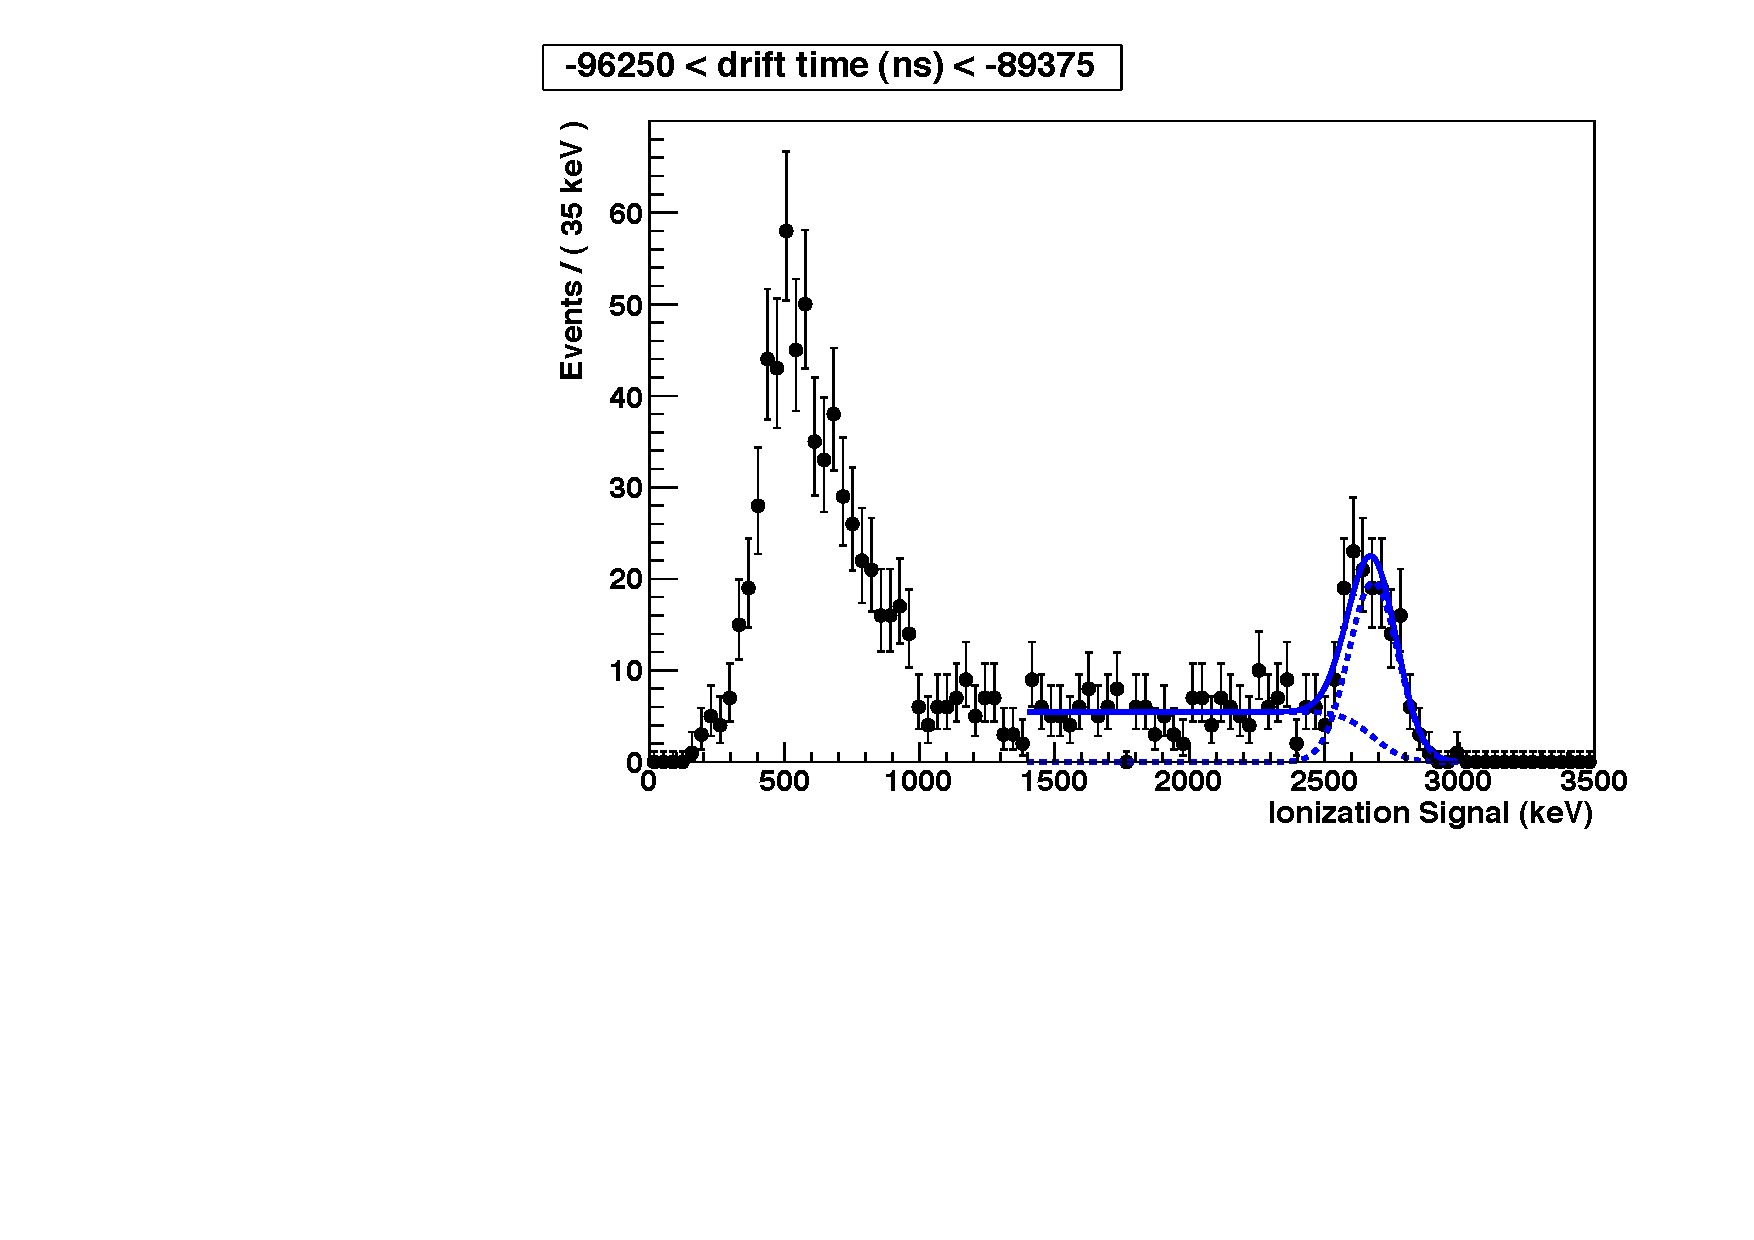
\includegraphics[width=0.8\columnwidth]{./plots/el_run4034_dt_bin_fit.pdf}
\caption[An example fit in a drift time bin]{A fit of the simple Gaussian + complementary error function model to one single drift time bin. In this example, the full absorption peak is the 2615 keV gamma line from \thorium{228}.}
\label{fig:dtbinfit}
\end{figure}

Plotting the full absorption peak energy from each drift time bin as a function of drift time reveals the exponential decay described in \cref{eq:exponentialtaue}. Fitting an exponential to each TPC yields a measurement of the electron lifetime for each. Alternatively, a fit with a single electron lifetime to the entire detector uses information from both TPCs. In all cases, the amplitude of the exponential is allowed to float in the fit, since only the relative decay matters when measuring the electron lifetime. Presently, the separate TPC lifetimes are used when correcting for electron lifetime in EXO-200, while the single measurement is used when monitoring the detector and data quality. \Cref{fig:elfit} shows an example.

\begin{figure}[htbp]
\centering
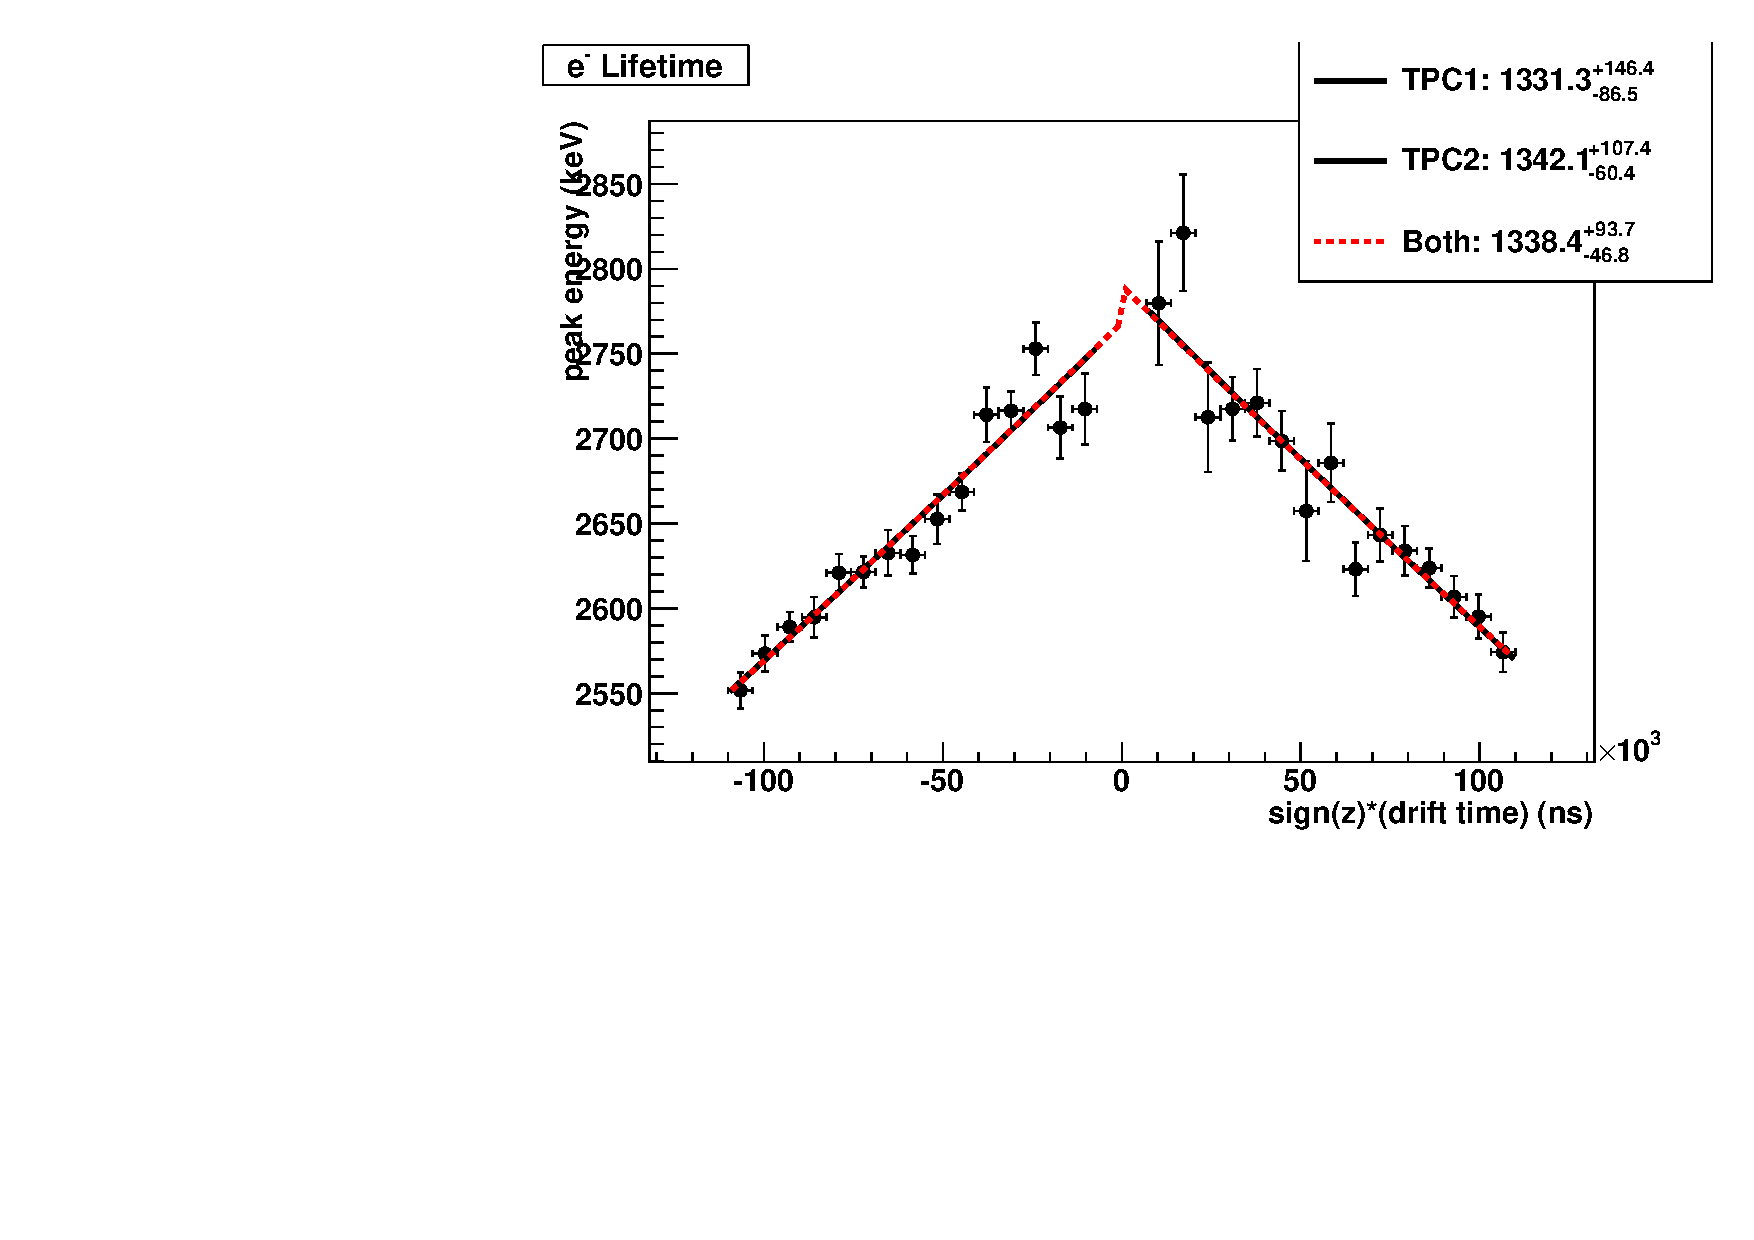
\includegraphics[width=0.8\columnwidth]{./plots/el_run4228_fit.pdf}
\caption[An example fit to exponential attenuation]{Measuring the electron lifetime by fitting a decaying exponential to the full-absorption peak energies binned by drift time. TPC 2 is assigned a negative drift time for convenience in visualization. Both fits to the individual TPCs and to both TPCs together are shown.}
\label{fig:elfit}
\end{figure}

The electron lifetime measurement comes from minimizing the \(\chi^2\) statistic. Confidence intervals for the measurement come from doing a profile scan. That is, the electron lifetime is set to some fixed value away from the best fix, and the amplitude is allowed to vary to minimize \(\chi^2\). All values for which \(\chi^2\) is less than 1 above the minimum value define the 1\(\sigma\) (68\%) confidence band. \Cref{fig:profileel} shows an example.

\begin{figure}[htbp]
\centering
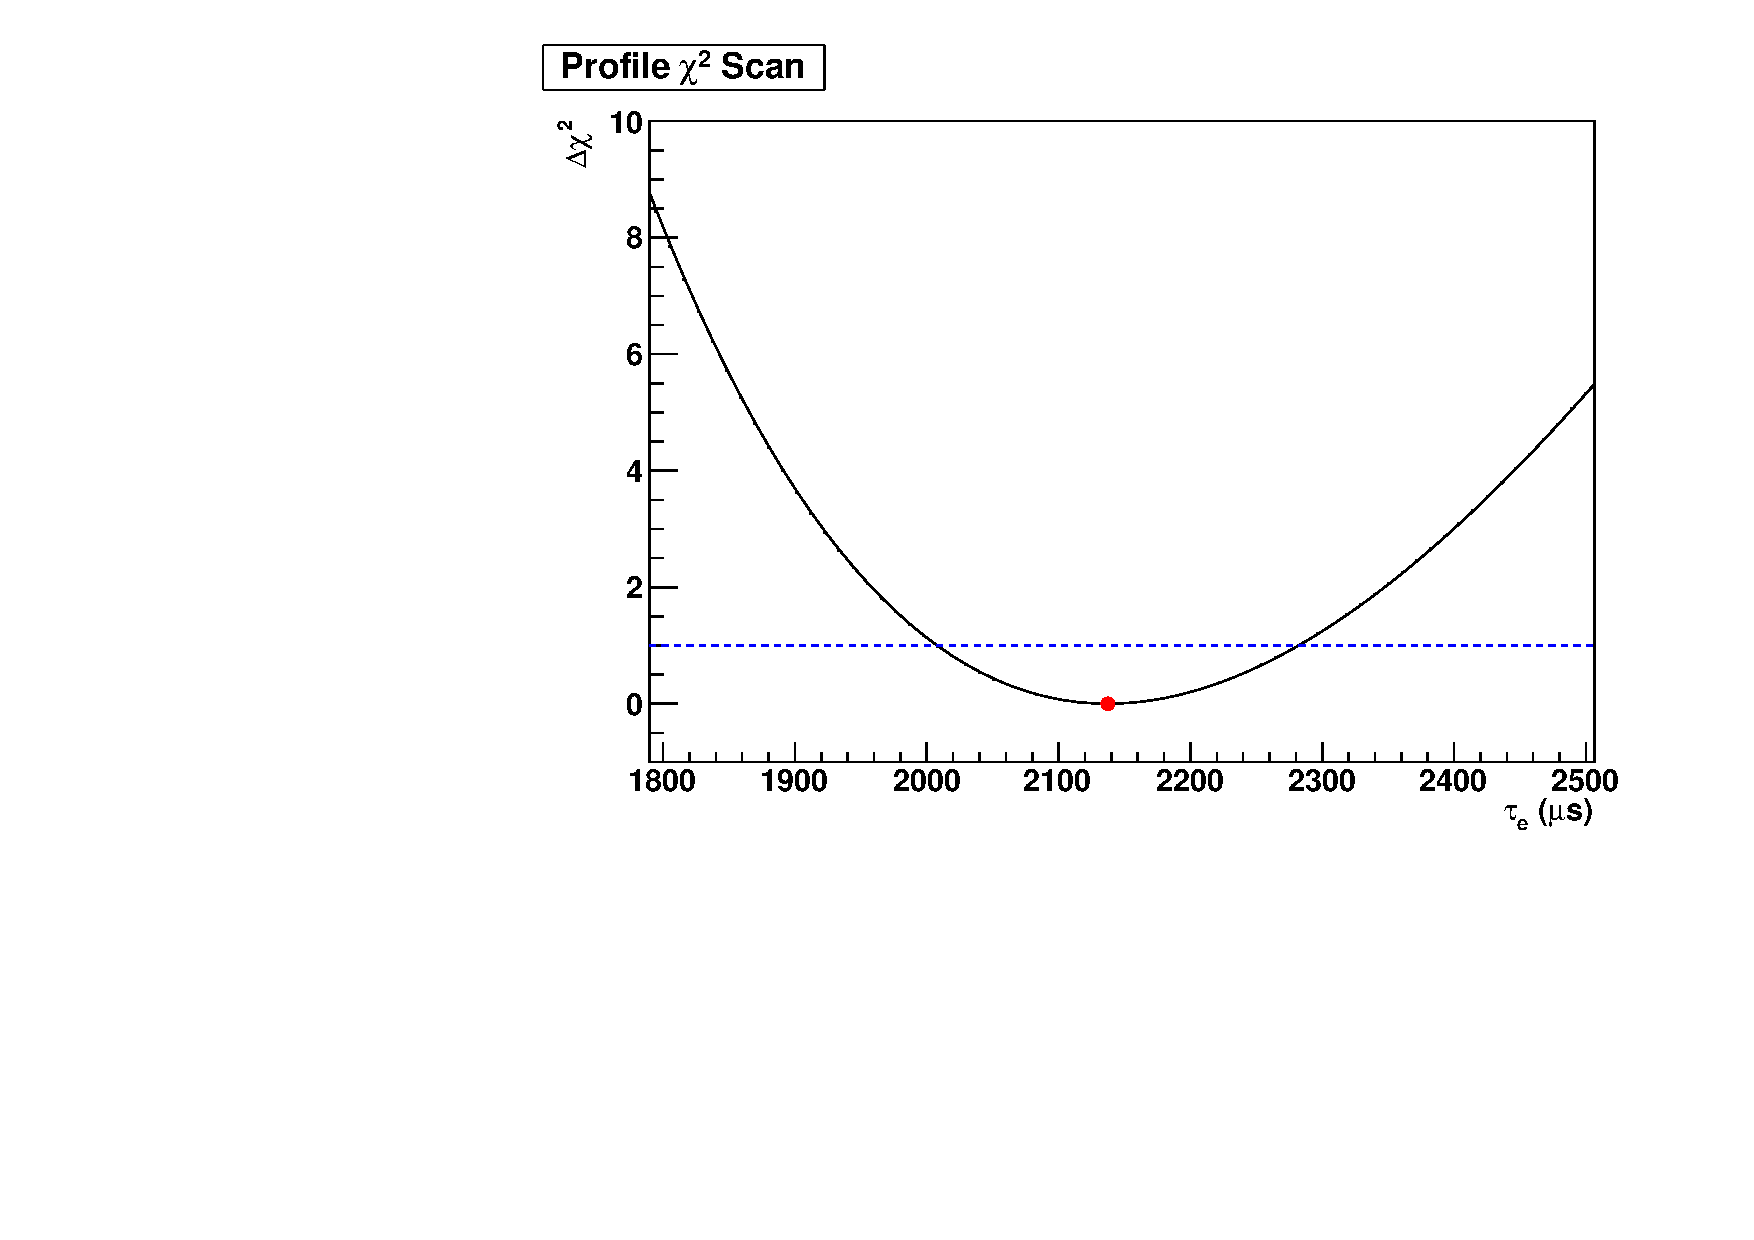
\includegraphics[width=0.8\columnwidth]{./plots/el_run4252_profile.pdf}
\caption[A profile scan around the best-fit electron lifetime]{Confidence intervals around the best fit electron lifetime come from a profile scan, shown here. As this figure shows, this is superior to simply estimating the 1\(\sigma\) errors from the second derivative at the best fit value, since the profile is asymmetric around the best fit (indicated by the red dot). The blue line indicates \(\Delta\chi^2 = 1\), corresponding to \(1\sigma\) errors.}
\label{fig:profileel}
\end{figure}

\subsection{Comparison to Simulation}

\subsection{Practical Considerations}

Energy resolution limits measurement of long electron lifetimes.

Statistical uncertainties on source peak location.

\section{Measurements of Electron Lifetime in EXO-200}

\subsection{Time Variation and Correction Function}

\subsection{Effects of Electron Lifetime on the Energy Resolution}

\subsection{Electron Lifetime in Low Electric Field}

\subsection{Comparison with Gas Purity Monitor Readings}

\end{document}